\documentclass{beamer}
\usepackage{graphicx}
\usepackage{verbatim}
\usepackage{amsmath}
\usepackage{amsfonts}
\usepackage{setspace}
% \usepackage{beamerthemesplit} // Activate for custom appearance

\title{Regression Estimation - Least
Squares and Maximum Likelihood}
\author{Dr. Frank Wood}

\date{}

\DeclareMathOperator*{\Ave}{\mathbb{E}}
\DeclareMathOperator*{\Var}{Var}

\begin{document}

\frame{\titlepage}

\frame[t] {
 \frametitle{Least Squares Max(min)imization}
 \begin{itemize}
\item Function to minimize w.r.t. $\beta_0, \beta_1$
$$Q = \sum_{i=1}^n (Y_i - (\beta_0 + \beta_1 X_i))^2$$
\item Minimize this by maximizing $-Q$
\item Find partials and set both equal to zero
\begin{eqnarray*}
\frac{dQ}{d\beta_0} &=& 0 \\
\frac{dQ}{d\beta_1} &=& 0
\end{eqnarray*}
\end{itemize}
}

\frame[t] {
 \frametitle{Normal Equations}
 \begin{itemize}
\item The result of this maximization step are called the normal equations.  $b_0$ and $b_1$ are called point estimators of $\beta_0$ and $\beta_1$
respectively.
\begin{eqnarray*}
\sum Y_i &=& nb_0 + b_1 \sum X_i \\
\sum X_iY_i &=& b_0 \sum X_i + b_1 \sum X_i^2
\end{eqnarray*}
\item This is a system of two equations and two unknowns.  The solution is given
by $\ldots$
\end{itemize}
}

\frame[t] {
 \frametitle{Solution to Normal Equations}
 After a lot of algebra one arrives at
 \begin{eqnarray*}
b_1 &=& \frac{\sum(X_i - \bar X)(Y_i - \bar Y)}{\sum(X_i-\bar X)^2} \\
b_0 &=& \bar Y - b_1 \bar X\\
\bar X &=& \frac{\sum X_i}{n} \\
\bar Y&=&\frac{\sum Y_i}{n}
\end{eqnarray*}

}

\frame[t] {%%%change pic%%%
 \frametitle{Least Squares Fit}
 \begin{figure}
  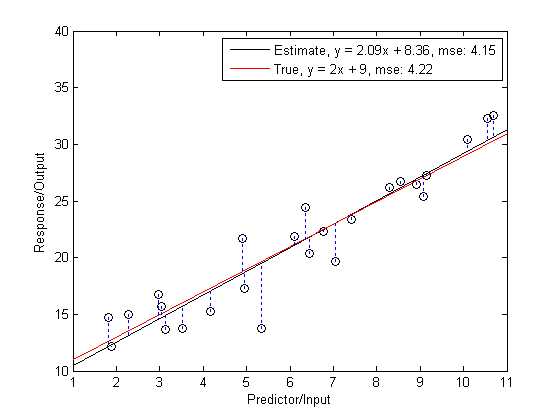
\includegraphics[height=60mm]{lsfit.png}
\end{figure}
}

\frame[t] {%%%change pic%%%
 \frametitle{Guess \#1}
 \begin{figure}
  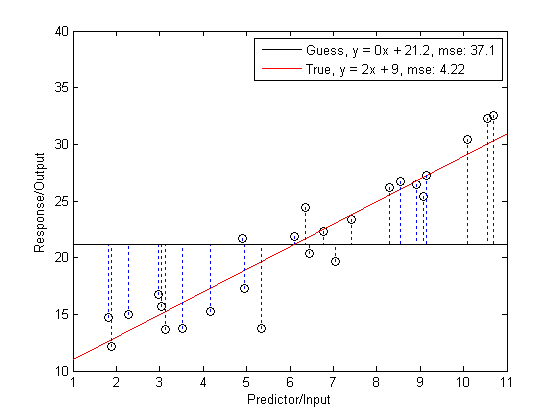
\includegraphics[height=60mm]{guess1.png}
\end{figure}
}

\frame[t] {%%%change pic%%%
 \frametitle{Guess \#2}
 \begin{figure}
  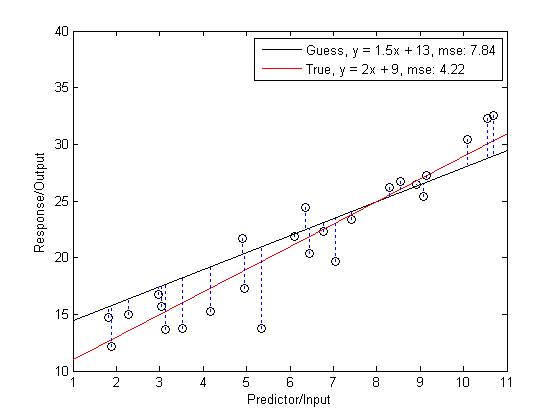
\includegraphics[height=60mm]{guess2.png}
\end{figure}
}

\frame[t] {
 \frametitle{Looking Ahead: Matrix Least Squares}
 $$\left[\begin{array}{c} Y_1 \\Y_2 \\ \vdots \\ Y_n \end{array} \right] =  \left[\begin{array}{cc} X_1 & 1\\X_2 & 1\\ {\vdots} \\ X_n & 1\end{array} \right]\left[ \begin{array}{cc} \beta_1 \\ \beta_0
 \end{array}\right]$$
 Solution to this equation is solution to least squares linear regression (and maximum likelihood under normal error distribution assumption)
}

\frame[t] {
 \frametitle{Questions to Ask}
 \begin{itemize}
\item Is the relationship really linear?
\item What is the distribution of the of ``errors''?
\item Is the fit good?
\item How much of the variability of the response is accounted for by including the predictor variable?
\item Is the chosen predictor variable the best one?
\end{itemize}
}

\frame[t] {%%%change pic%%%
 \frametitle{Is This Better?}
  \begin{figure}
  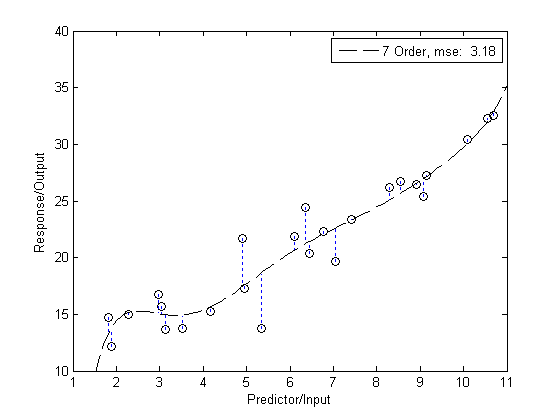
\includegraphics[height=60mm]{better.png}
\end{figure}
}

\frame[t] {
 \frametitle{Goals for First Half of Course}
 \begin{itemize}
\item How to do linear regression
\begin{itemize}
\item Self familiarization with software tools
\end{itemize}
\item How to interpret standard linear regression results
\item How to derive tests
\item How to assess and address deficiencies in regression models
\end{itemize}
}

\frame[t] {
 \frametitle{Estimators for $\beta_0, \beta_1, \sigma^2$}
 \begin{itemize}
\item We want to establish properties of estimators for $\beta_0, \beta_1,$ and $\sigma^2$ so that we can construct hypothesis tests and so forth
\item We will start by establishing some properties of the regression solution.
\end{itemize}
}

\frame[t] {
 \frametitle{Properties of Solution}
 \begin{itemize}
\item The $i^{th}$ residual is defined to be
$$e_i = Y_i - \hat Y_i$$
\item The sum of the residuals is zero:
\begin{eqnarray*}
\sum_i e_i &=& \sum(Y_i -b_0 -b_1 X_i) \\
&=& \sum Y_i - n b_0 - b_1 \sum X_i \\
&=& 0
\end{eqnarray*}
\end{itemize}
}

\frame[t] {
 \frametitle{Properties of Solution}
 The sum of the observed values $Y_i$ equals the sum of the fitted
 values $\widehat{Y}_i$
\begin{eqnarray*}
\sum_i Y_i &=& \sum_i \hat Y_i \\
&=& \sum_i  (b_1X_i + b_0) \\
&=& \sum_i (b_1X_i + \bar Y - b_1\bar X) \\
&=& b_1 \sum_i X_i + n \bar Y -b_1 n \bar X \\
&=& b_1 n \bar X + \sum_i Y_i -b_1 n \bar X
\end{eqnarray*}

}

\frame[t] {
 \frametitle{Properties of Solution}
The sum of the weighted residuals is zero when the residual in the
$i^{th}$ trial is weighted by the level of the predictor variable in
the $i^{th}$ trial
\begin{eqnarray*}
\sum_i X_i e_i &=& \sum(X_i(Y_i -b_0 -b_1X_i))\\
&=& \sum_i X_iY_i - b_0 \sum X_i - b_1 \sum (X_i^2)\\
&=& 0
\end{eqnarray*}

}

\frame[t] {
 \frametitle{Properties of Solution}
The regression line always goes through the point
$$\bar X, \bar Y$$
}

\frame[t] {
 \frametitle{Estimating Error Term Variance $\sigma^2$}
 \begin{itemize}
\item Review estimation in non-regression setting.
\item Show estimation results for regression setting.
\end{itemize}
}

\frame[t] {
 \frametitle{Estimation Review}
\begin{itemize}
\item An estimator is a rule that tells how to calculate the value of an estimate based on the measurements contained in a sample

\item i.e. the sample mean
$$\bar Y = \frac{1}{n} \sum_{i=1}^{n} Y_i$$
\end{itemize}
}

\frame[t] {
 \frametitle{Point Estimators and Bias}
\begin{itemize}
\item Point estimator
$$\hat \theta = f(\{ Y_1, \ldots, Y_n\})$$
\item Unknown quantity / parameter
$$\theta$$
\item Definition: Bias of estimator
$$B(\hat \theta) = \Ave(\hat \theta) - \theta$$
\end{itemize}
}

\frame[t] {%%%change pic%%%
 \frametitle{One Sample Example}
\begin{figure}
  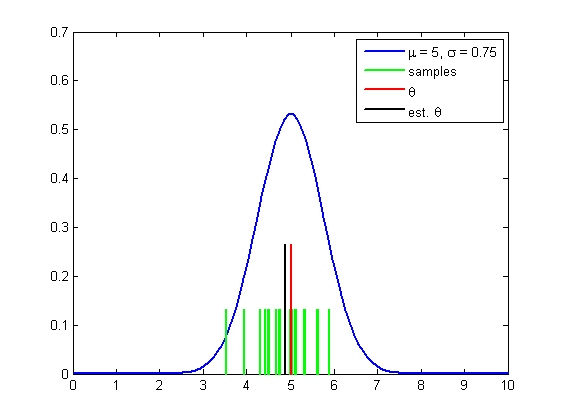
\includegraphics[height=60mm]{onesample.png}
\end{figure}
}

\frame[t] {
 \frametitle{Distribution of Estimator}
\begin{itemize}
\item If the estimator is a function of the samples and the distribution of the samples is known then the distribution of the estimator can (often) be determined
\begin{itemize}
\item Methods
\begin{itemize}
\item Distribution (CDF) functions
\item Transformations
\item Moment generating functions
\item Jacobians (change of variable)
\end{itemize}
\end{itemize}
\end{itemize}
}

\frame[t] {
 \frametitle{Example}
\begin{itemize}
\item Samples from a $Normal(\mu,\sigma^2)$ distribution
$$Y_i \sim \mathrm{Normal}(\mu,\sigma^2)$$
\item Estimate the population mean
$$\theta = \mu, \quad \hat \theta = \bar Y = \frac{1}{n} \sum_{i=1}^{n} Y_i$$
\end{itemize}
}

\frame[t] {
 \frametitle{Sampling Distribution of the Estimator}
\begin{itemize}
\item First moment
\begin{eqnarray*}
\Ave(\hat \theta) &=& \Ave(\frac{1}{n} \sum_{i=1}^{n} Y_i) \\
&=& \frac{1}{n} \sum_{i=1}^{n} \Ave(Y_i) = \frac{n\mu}{n} = \theta
\end{eqnarray*}
\item This is an example of an unbiased estimator
$$B(\hat \theta) = \Ave(\hat \theta) - \theta = 0$$
\end{itemize}
}

\frame[t] {
 \frametitle{Variance of Estimator}
\begin{itemize}
\item Definition: Variance of estimator
$$\Var(\hat \theta) = \Ave([\hat \theta - \Ave(\hat \theta)]^2)$$
\item Remember:
\begin{eqnarray*}
\Var(cY) &=& c^2\Var(Y)\\
\Var(\sum_{i=1}^n Y_i) &=& \sum_{i=1}^n\Var(Y_i)
\end{eqnarray*}
Only if the $Y_i$ are independent with finite variance

\end{itemize}
}

\frame[t] {
 \frametitle{Example Estimator Variance}
\begin{itemize}
\item For $N(0,1)$ mean estimator
\begin{eqnarray*}
\Var(\hat \theta) &=& \Var(\frac{1}{n} \sum_{i=1}^{n} Y_i) \\
&=& \frac{1}{n^2} \sum_{i=1}^{n} \Var(Y_i) = \frac{n\sigma^2}{n^2} =
\frac{\sigma^2}{n}
\end{eqnarray*}

\item Note assumptions
\end{itemize}
}

\frame[t] {
 \frametitle{Central Limit Theorem Review}
\begin{block}{Central Limit Theorem}
Let $Y_1, Y_2, \ldots, Y_n$ be iid random variables with $\Ave(Y_i) = \mu$ and $\Var(Y_i) - \sigma^2 < \infty$.  Define.
\begin{equation}
U_n = \sqrt{n}\left(\frac{\bar Y - \mu}{\sigma}\right) \;\;\; \mbox{where} \;\;\;  \bar Y = \frac{1}{n}\sum_{i=1}^n Y_i
\end{equation}
Then the distribution function of $U_n$ converges to a standard normal distribution function as $n\rightarrow\infty$.
\end{block}

\begin{block}{Alternately}
\begin{equation}
P(a\leq U_n\leq b) \rightarrow \int_a^b \left(\frac{1}{\sqrt{2\pi}}\right) e^{\frac{-u^2}{2}}du
\end{equation}
\end{block}
}


\frame[t] {%%%change pic%%%
 \frametitle{Distribution of sample mean estimator}
\begin{figure}
  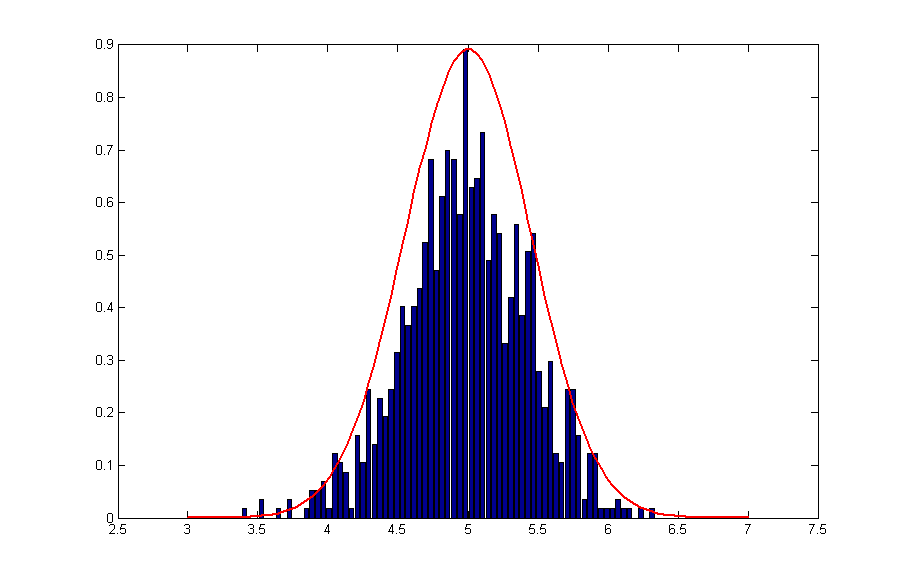
\includegraphics[height=60mm]{mean.png}
\end{figure}
}

\frame[t] {
 \frametitle{Bias Variance Trade-off}
\begin{itemize}
\item The mean squared error of an estimator
$$MSE(\hat \theta) = \Ave([\hat \theta -  \theta]^2)$$
\item Can be re-expressed
$$MSE(\hat \theta) = \Var(\hat \theta) + (B( \hat \theta)^2)$$
\end{itemize}
}

\frame[t] {
 \frametitle{MSE = VAR + $BIAS^2$}
 Proof
\begin{eqnarray*}
MSE(\hat \theta) &=& \Ave((\hat \theta - \theta)^2) \\
&=& \Ave(([\hat \theta -\Ave(\hat \theta)]+ [\Ave(\hat \theta)-\theta])^2) \\
&=& \Ave([\hat \theta -\Ave(\hat \theta)]^2) + 2\Ave([\Ave(\hat \theta)-\theta][\hat \theta - \Ave(\hat \theta)]) + \Ave([\Ave(\hat \theta) - \theta]^2) \\
&=& \Var(\hat \theta) + 2  \Ave([\Ave(\hat \theta)[\hat \theta - \Ave(\hat \theta)] - \theta[\hat \theta - \Ave(\hat \theta)]))  + (B(\hat \theta))^2\\
&=& \Var(\hat \theta) + 2 (0 + 0) +  (B(\hat \theta))^2 \\
&=& \Var(\hat \theta) + (B(\hat \theta))^2 \\
\end{eqnarray*}

}

\frame[t] {
 \frametitle{Trade-off}
\begin{itemize}
\item Think of variance as confidence and bias as correctness.
\begin{itemize}
\item Intuitions (largely) apply
\end{itemize}
\item Sometimes choosing a biased estimator can result in an overall lower MSE if it exhibits lower variance.
\item Bayesian methods (later in the course) specifically introduce bias.
\end{itemize}
}

\frame[t] {
 \frametitle{Estimating Error Term Variance $\sigma^2$}
\begin{itemize}
\item Regression model
\item Variance of each observation $Y_i$ is $\sigma^2$ (the same as for the error term $\epsilon_i$)
\item Each $Y_i$ comes from a different probability distribution with different means that depend on the level
$X_i$
\item The deviation of an observation $Y_i$ must be calculated around its own estimated mean.
\end{itemize}
}

\frame[t] {
 \frametitle{$s^2$ estimator for $\sigma^2$}
$$s^2 = MSE = \frac{SSE}{n-2} = \frac{\sum(Y_i-\hat Y_i)^2}{n-2} = \frac{\sum e_i^2} {n-2}$$
\begin{itemize}
\item MSE is an unbiased estimator of $\sigma^2$
$$\Ave(MSE) = \sigma^2$$
\item The sum of squares SSE has n-2 ``degrees of freedom'' associated with it.
\item Cochran's theorem (later in the course) tells us where degree's of freedom come from and how to calculate them.
\end{itemize}
}

\frame[t] {
 \frametitle{Normal Error Regression Model}
\begin{itemize}
\item No matter how the error terms $\epsilon_i$ are distributed, the least squares method provides unbiased point estimators of $\beta_0$ and
$\beta_1$
\begin{itemize}
\item that also have minimum variance among all unbiased linear estimators
\end{itemize}
\item To set up interval estimates and make tests we need to specify the distribution of the $\epsilon_i$
\item We will assume that the $\epsilon_i$ are normally distributed.
\end{itemize}
}

\frame[t] {
 \frametitle{Normal Error Regression Model}
$$Y_i = \beta_0 + \beta_1 X_i + \epsilon_i$$
\begin{itemize}
\item $Y_i$ value of the response variable in the $i^{th}$ trial
\item $\beta_0$ and $\beta_1$ are parameters
\item $X_i$ is a known constant, the value of the predictor variable in the $i^{th}$ trial
\item $\epsilon_i \sim_{iid} N(0,\sigma^2)$ \\{\em note this is different, now we know the distribution}
\item $i = 1,\ldots,n$
\end{itemize}
}

\frame[t] {
 \frametitle{Notational Convention}
\begin{itemize}
\item When you see $\epsilon_i \sim_{iid} N(0,\sigma^2)$
\item It is read as $\epsilon_i$ is distributed identically and independently according to a normal distribution with mean 0 and variance
$\sigma^2$
\item Examples
\begin{itemize}
\item $\theta \sim Poisson(\lambda)$
\item $z \sim G(\theta)$
\end{itemize}
\end{itemize}
}

\frame[t] {
 \frametitle{Maximum Likelihood Principle}
The method of maximum likelihood chooses as estimates those values
of the parameters that are most consistent with the sample data. }

\frame[t] {
 \frametitle{Likelihood Function}
If $$X_i \sim F(\Theta), i=1\ldots n$$ then the likelihood function
is
$$\mathcal{L}(\{X_i\}_{i=1}^n, \Theta) =  \prod_{i=1}^n F(X_i;
\Theta)$$}


\frame[t] {%%%change pic%%%
 \frametitle{Example, $N(10,3)$ Density, Single Obs.}
\begin{figure}
  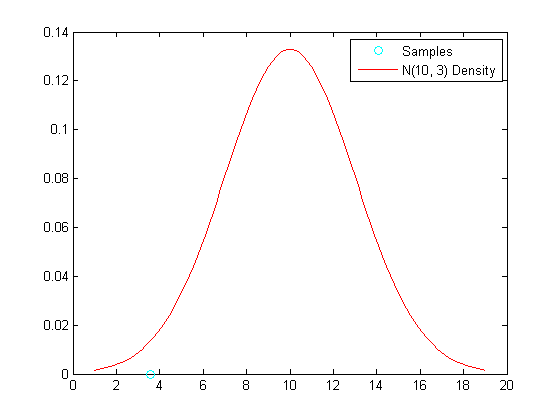
\includegraphics[height=60mm]{n103.png}
\end{figure}
}

\frame[t] {%%%change pic%%%
 \frametitle{Example, $N(10,3)$ Density, Single Obs. Again}
\begin{figure}
  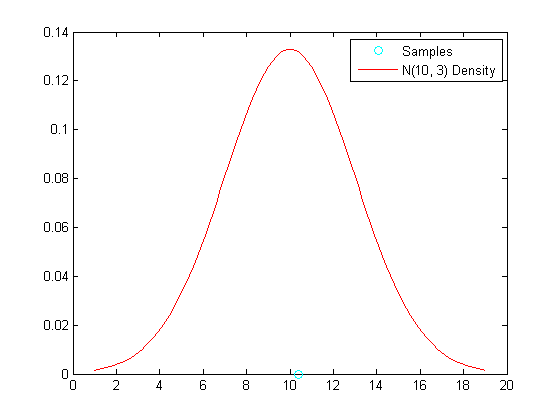
\includegraphics[height=60mm]{n103a.png}
\end{figure}
}

\frame[t] {%%%change pic%%%
 \frametitle{Example, $N(10,3)$ Density, Multiple Obs.}
\begin{figure}
  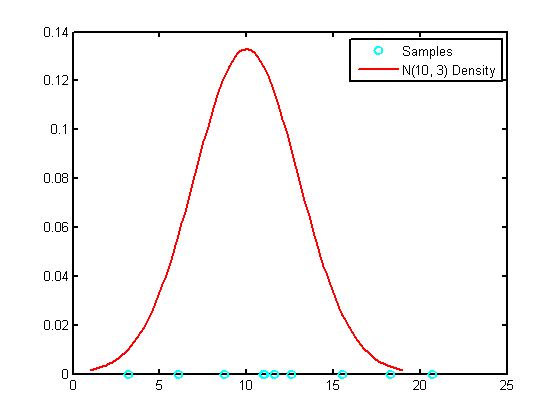
\includegraphics[height=60mm]{n103m.png}
\end{figure}
}

\frame[t] {
 \frametitle{Maximum Likelihood Estimation}
\begin{itemize}
\item The likelihood function can be maximized w.r.t. the parameter(s) $\Theta$, doing this one can arrive at estimators for parameters as well.
$$\mathcal{L}(\{X_i\}_{i=1}^n, \Theta) =  \prod_{i=1}^n F(X_i; \Theta)$$
\item To do this, find solutions to (analytically or by following gradient)
$$\frac{d\mathcal{L}(\{X_i\}_{i=1}^n, \Theta)}{d\Theta} = 0$$
\end{itemize}
}

\frame[t] {
 \frametitle{Important Trick}
Never (almost) maximize the likelihood function, maximize the $\log$
likelihood function instead.
\begin{eqnarray*}
log (\mathcal{L}(\{X_i\}_{i=1}^n, \Theta)) &=&  log (\prod_{i=1}^n F(X_i; \Theta))\\
&=& \sum_{i=1}^n log(F(X_i; \Theta))
\end{eqnarray*}
Quite often the log of the density is easier to work with
mathematically. }

\frame[t] {
 \frametitle{ML Normal Regression}
Likelihood function
\begin{eqnarray*}
\mathcal{L}(\beta_0, \beta_1, \sigma^2) &=& \prod_{i=1}^n \frac{1}{(2\pi\sigma^2)^{1/2}} e^{-\frac{1}{2\sigma^2} (Y_i - \beta_0 -\beta_1X_i)^2} \\
&=&  \frac{1}{(2\pi\sigma^2)^{n/2}} e^{-\frac{1}{2\sigma^2}
\sum_{i=1}^n (Y_i - \beta_0 -\beta_1X_i)^2}
\end{eqnarray*}
which if you maximize (how?) w.r.t. to the parameters you
get$\ldots$}

\frame[t] {
 \frametitle{Maximum Likelihood Estimator(s)}
\begin{itemize}
\item $\beta_0$\\$b_0$ same as in least squares case
\item $\beta_1$\\$b_1$ same as in least squares case
\item $\sigma_2$\\ $$\hat \sigma^2 = \frac{\sum_i(Y_i-\hat Y_i)^2}{n}$$
\item Note that ML estimator is biased as $s^2$ is unbiased and
$$s^2 = MSE =  \frac{n}{n-2} \hat \sigma^2$$
\end{itemize}
}

\frame[t] {
 \frametitle{Comments}
\begin{itemize}
\item Least squares minimizes the squared error between the prediction and the true output
\item The normal distribution is fully characterized by its first two central moments (mean and variance)
\item Food for thought:
\begin{itemize}
\item What does the bias in the ML estimator of the error variance mean?  And where does it come from?

\end{itemize}
\end{itemize}
}


\end{document}
